\documentclass[9pt,aspectratio=169]{beamer}
\usetheme{Madrid}

% ─── Кодировка и язык ────────────────────────────────────────────────────────
\usepackage[T2A]{fontenc}
\usepackage[utf8]{inputenc}
\usepackage[russian]{babel}

\usepackage{graphicx}
\usepackage{amsmath,amssymb}
\usepackage{tikz}
\usetikzlibrary{arrows.meta, positioning}

% ─── Цветовая схема: тёмный серо-графитовый ──────────────────────────────────
\definecolor{Graphite}{RGB}{55, 58, 64}
\definecolor{GraphiteDark}{RGB}{33, 35, 40}
\definecolor{GraphiteLight}{RGB}{240, 241, 243}
\definecolor{GraphiteAccent}{RGB}{180, 60, 45}

\usecolortheme[named=Graphite]{structure}

\setbeamercolor{palette primary}    {bg=Graphite,       fg=white}
\setbeamercolor{palette secondary}  {bg=GraphiteDark,   fg=white}
\setbeamercolor{palette tertiary}   {bg=GraphiteDark,   fg=white}
\setbeamercolor{palette quaternary} {bg=Graphite,       fg=white}
\setbeamercolor{titlelike}          {bg=Graphite,       fg=white}
\setbeamercolor{block title}        {bg=Graphite,       fg=white}
\setbeamercolor{block body}         {bg=GraphiteLight,  fg=black}
\setbeamercolor{block title alerted}{bg=GraphiteAccent, fg=white}
\setbeamercolor{block body alerted} {bg=GraphiteLight,  fg=black}
\setbeamercolor{alerted text}       {fg=GraphiteAccent}

% ─── Метаданные ──────────────────────────────────────────────────────────────
\title{Численное моделирование флаттера упругого крыла}
\author{Александр Лебедев, Смола Максим}
\institute{Московский физико-технический институт}
\date{\today}

% ─────────────────────────────────────────────────────────────────────────────
\begin{document}

% ══════════════════════════════════════════════════════════════════════════════
% СЛАЙД 1 — ТИТУЛ
% ══════════════════════════════════════════════════════════════════════════════
{
\setbeamertemplate{headline}{}
\begin{frame}
  \titlepage
\end{frame}
}

% ══════════════════════════════════════════════════════════════════════════════
\section{Проблема: аэроупругий флаттер}
% ══════════════════════════════════════════════════════════════════════════════

\begin{frame}{Что такое флаттер?}
  \begin{block}{Определение}
    Флаттер~--- \alert{самовозбуждающиеся колебания} конструкции
    без внешнего воздействия, возникающие из-за взаимодействия
    аэродинамических, упругих и инерционных сил.
  \end{block}

  \medskip

  \begin{columns}[T]
    \column{0.48\textwidth}
      \begin{block}{Режимы поведения}
        \begin{itemize}
          \item $U < U_{\mathrm{crit}}$: колебания \textbf{затухают}
          \item $U \approx U_{\mathrm{crit}}$: \textbf{устойчивые} осцилляции
          \item $U > U_{\mathrm{crit}}$: \alert{дивергентный флаттер}
        \end{itemize}
      \end{block}

    \column{0.48\textwidth}
      \begin{alertblock}{Последствия}
        Рост амплитуды $\Rightarrow$ рост напряжений $\Rightarrow$
        усталость $\Rightarrow$ \alert{разрушение конструкции}.
      \end{alertblock}
  \end{columns}
\end{frame}

% ══════════════════════════════════════════════════════════════════════════════
\section{Постановка задачи}
% ══════════════════════════════════════════════════════════════════════════════

\begin{frame}{Постановка задачи}
  \begin{columns}[T]
    \column{0.50\textwidth}
      \begin{block}{Система координат}
        \begin{itemize}
          \item $X$~--- направление потока
          \item $Y$~--- размах крыла
          \item $Z$~--- вертикальное направление
        \end{itemize}
        \[
          \mathbf{U}_\infty = (U,\;0,\;0)
        \]
      \end{block}

      \medskip

      \begin{block}{Модель}
        \begin{itemize}
          \item Корень ($y=0$) \textbf{жёстко закреплён}
          \item Две степени свободы: изгиб $q_b$ и кручение $q_t$
        \end{itemize}
      \end{block}

    \column{0.46\textwidth}
      \begin{block}{Обобщённые координаты}
        \[
          \mathbf{q}(t) = \begin{bmatrix} q_b(t) \\ q_t(t) \end{bmatrix}
        \]
        Полный CFD/FEM~--- миллионы DOF.
        Две координаты воспроизводят все три режима флаттера
        при минимальных вычислительных затратах.
      \end{block}
  \end{columns}
\end{frame}

\begin{frame}{Тетраэдральная сетка крыла}
  \begin{center}
    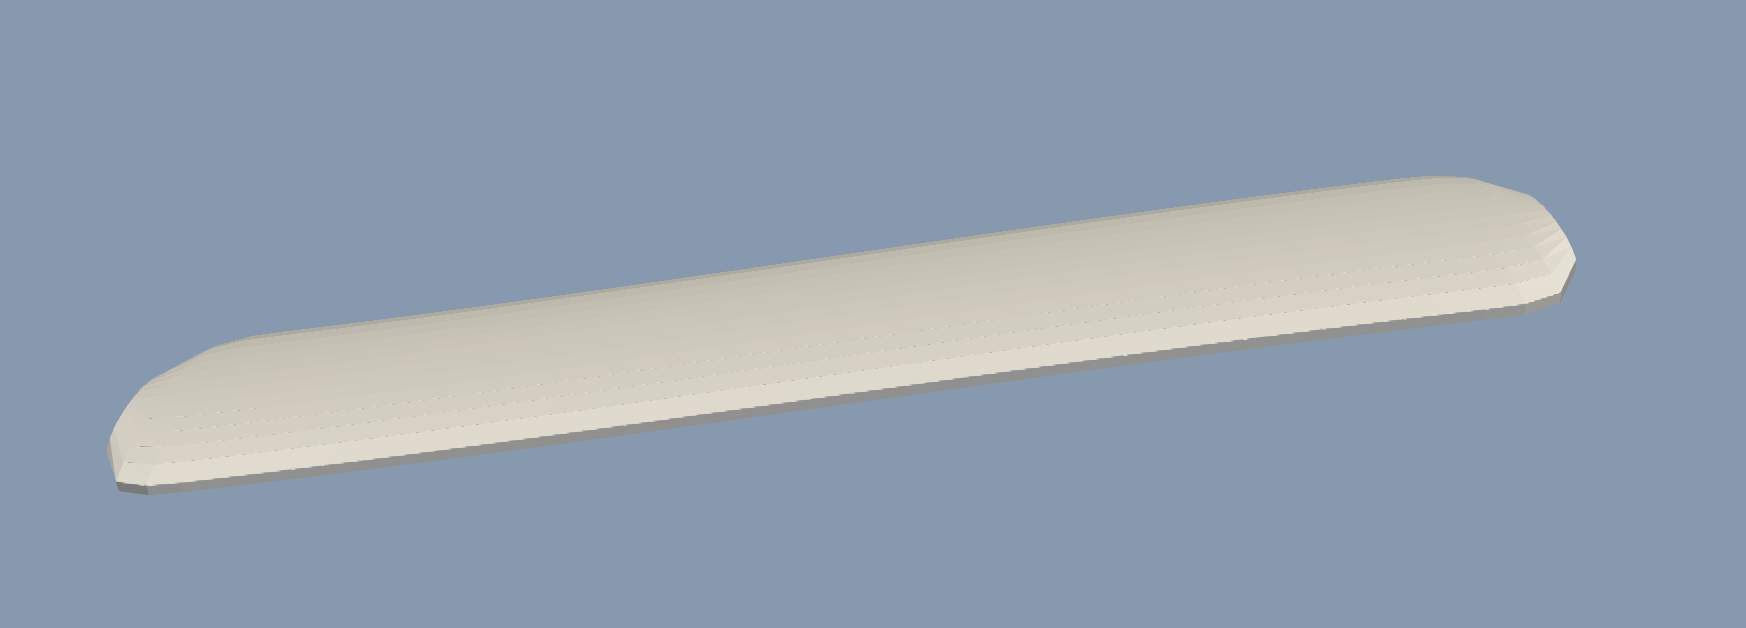
\includegraphics[width=0.72\linewidth]{../images/mesh.png}\\[6pt]
    \small Тетраэдральная FEM-сетка, сгенерированная в Gmsh
  \end{center}
\end{frame}

% ══════════════════════════════════════════════════════════════════════════════
\section{Физическая модель}
% ══════════════════════════════════════════════════════════════════════════════

\begin{frame}{Модальные формы: изгиб и кручение}
  \begin{columns}[T]
    \column{0.48\textwidth}
      \begin{block}{Изгиб (Bending)}
        \[
          w(y,t) = q_b(t)\,\phi_b(y)
        \]
        Консольная форма ($\xi = -y/L$):
        \[
          \phi_b(\xi) = \xi^2(3 - 2\xi)
        \]
        $\phi_b(0)=0$~--- заделка, \; $\phi_b(1)=1$~--- конец.
      \end{block}

    \column{0.48\textwidth}
      \begin{block}{Кручение (Torsion)}
        \[
          \theta(y,t) = q_t(t)\,\phi_t(y)
        \]
        Форма: $\phi_t(\xi) = \xi$ или $\xi^2$.

        \medskip
        Кинематика малых углов:
        \[
          x' = x + z\theta, \quad z' = z - x\theta
        \]
      \end{block}
  \end{columns}

  \medskip

  \begin{alertblock}{Роль кручения}
    Кручение изменяет местный угол атаки~--- это \alert{главная причина}
    нестабилизирующего аэродинамического момента и флаттера.
  \end{alertblock}
\end{frame}

\begin{frame}{Уравнения движения}
  \begin{block}{Система Лагранжа II рода}
    \[
      M\,\ddot{\mathbf{q}} + C\,\dot{\mathbf{q}} + K\,\mathbf{q}
      = \mathbf{Q}_{\mathrm{aero}}
    \]
  \end{block}

  \medskip

  \begin{columns}[T]
    \column{0.32\textwidth}
      \begin{block}{Масса}
        \[
          M = \begin{bmatrix} m_b & 0 \\ 0 & I_t \end{bmatrix}
        \]
      \end{block}

    \column{0.32\textwidth}
      \begin{block}{Демпфирование}
        \[
          C = \begin{bmatrix} c_b & 0 \\ 0 & c_t \end{bmatrix}
        \]
      \end{block}

    \column{0.32\textwidth}
      \begin{block}{Жёсткость}
        \[
          K = \begin{bmatrix} k_b & 0 \\ 0 & k_t \end{bmatrix}
        \]
      \end{block}
  \end{columns}

  \medskip

  \begin{block}{Интегрирование~--- явный метод Эйлера}
    \[
      \dot{\mathbf{q}}^{n+1} = \dot{\mathbf{q}}^{n} + \Delta t\,\ddot{\mathbf{q}}^{n},
      \qquad
      \mathbf{q}^{n+1} = \mathbf{q}^{n} + \Delta t\,\dot{\mathbf{q}}^{n}
    \]
  \end{block}
\end{frame}

% ══════════════════════════════════════════════════════════════════════════════
\section{Аэродинамика и механизм флаттера}
% ══════════════════════════════════════════════════════════════════════════════

\begin{frame}{Аэродинамическая модель}
  \begin{columns}[T]
    \column{0.50\textwidth}
      \begin{block}{Эффективный угол атаки}
        \[
          \alpha_{\mathrm{eff}}
          = \theta + \frac{-\dot{w} + x\dot{\theta}}{U}
        \]
        Учитывает кручение, скорость изгиба и вращение
        профиля~--- \alert{главный механизм флаттера}.
      \end{block}

      \begin{block}{Динамическое давление}
        \[
          q_\infty = \tfrac{1}{2}\rho U^2
        \]
      \end{block}

    \column{0.46\textwidth}
      \begin{block}{Аэродинамическое запаздывание}
        \[
          \tau_a\,\dot{\alpha}_{\mathrm{lag}} + \alpha_{\mathrm{lag}}
          = \alpha_{\mathrm{eff}}
        \]
        \[
          C_L = C_{L\alpha}\,\alpha_{\mathrm{lag}}
        \]
        Моделирует \alert{отрицательное демпфирование}.
      \end{block}

      \begin{block}{Аэродинамический момент}
        \[
          M_y = -(x - x_{\mathrm{ac}})\,L
        \]
      \end{block}
  \end{columns}
\end{frame}

\begin{frame}{Механизм флаттера: замкнутая обратная связь}
  \vspace{0.4em}
  \begin{center}
  \begin{tikzpicture}[
      node distance=0.45cm and 1.8cm,
      box/.style={draw=Graphite, fill=GraphiteLight,
                  rounded corners=3pt, font=\small,
                  text width=3.3cm, align=center, minimum height=0.60cm},
      arr/.style={-{Stealth[length=5pt]}, Graphite, thick}
    ]
    \node[box] (wb)   {Скорость изгиба $\dot{w}$};
    \node[box, below=of wb]   (ae)   {$\alpha_{\mathrm{eff}}$~--- эфф. угол атаки};
    \node[box, below=of ae]   (lift) {Изменение подъёмной силы $\Delta L$};
    \node[box, below=of lift] (mom)  {Аэродинамический момент $M_y$};
    \node[box, right=2.6cm of mom]  (tor)  {Кручение $\theta$};
    \node[box, above=of tor]  (dL)   {Дополнительная $\Delta L$};
    \node[box, above=of dL, draw=GraphiteAccent]
                              (grow) {\alert{Рост колебаний}};

    \foreach \a/\b in {wb/ae, ae/lift, lift/mom, mom/tor, tor/dL, dL/grow}
      \draw[arr] (\a) -- (\b);

    \draw[arr, dashed, GraphiteAccent, bend left=55]
      (grow.north) to node[above, font=\scriptsize]{обратная связь} (wb.north);
  \end{tikzpicture}
  \end{center}
\end{frame}

% ══════════════════════════════════════════════════════════════════════════════
\section{Напряжения и алгоритм}
% ══════════════════════════════════════════════════════════════════════════════

\begin{frame}{Расчёт напряжений в тетраэдрах}
  \begin{columns}[T]
    \column{0.50\textwidth}
      \begin{block}{Изгибные напряжения}
        \[
          \sigma = E\,z\,\kappa
        \]
        $E$~--- модуль Юнга, \; $\kappa$~--- кривизна оси.
      \end{block}

      \begin{block}{Касательные напряжения}
        \[
          \tau = G\,r\,\frac{\partial\theta}{\partial y}
        \]
        $G$~--- модуль сдвига, \; $r$~--- расстояние до оси.
      \end{block}

      \begin{alertblock}{Критерий Мизеса}
        \[
          \sigma_{\mathrm{eq}} = \sqrt{\sigma^2 + 3\tau^2}
        \]
        Растёт неограниченно при флаттере.
      \end{alertblock}

    \column{0.46\textwidth}
      \begin{center}
        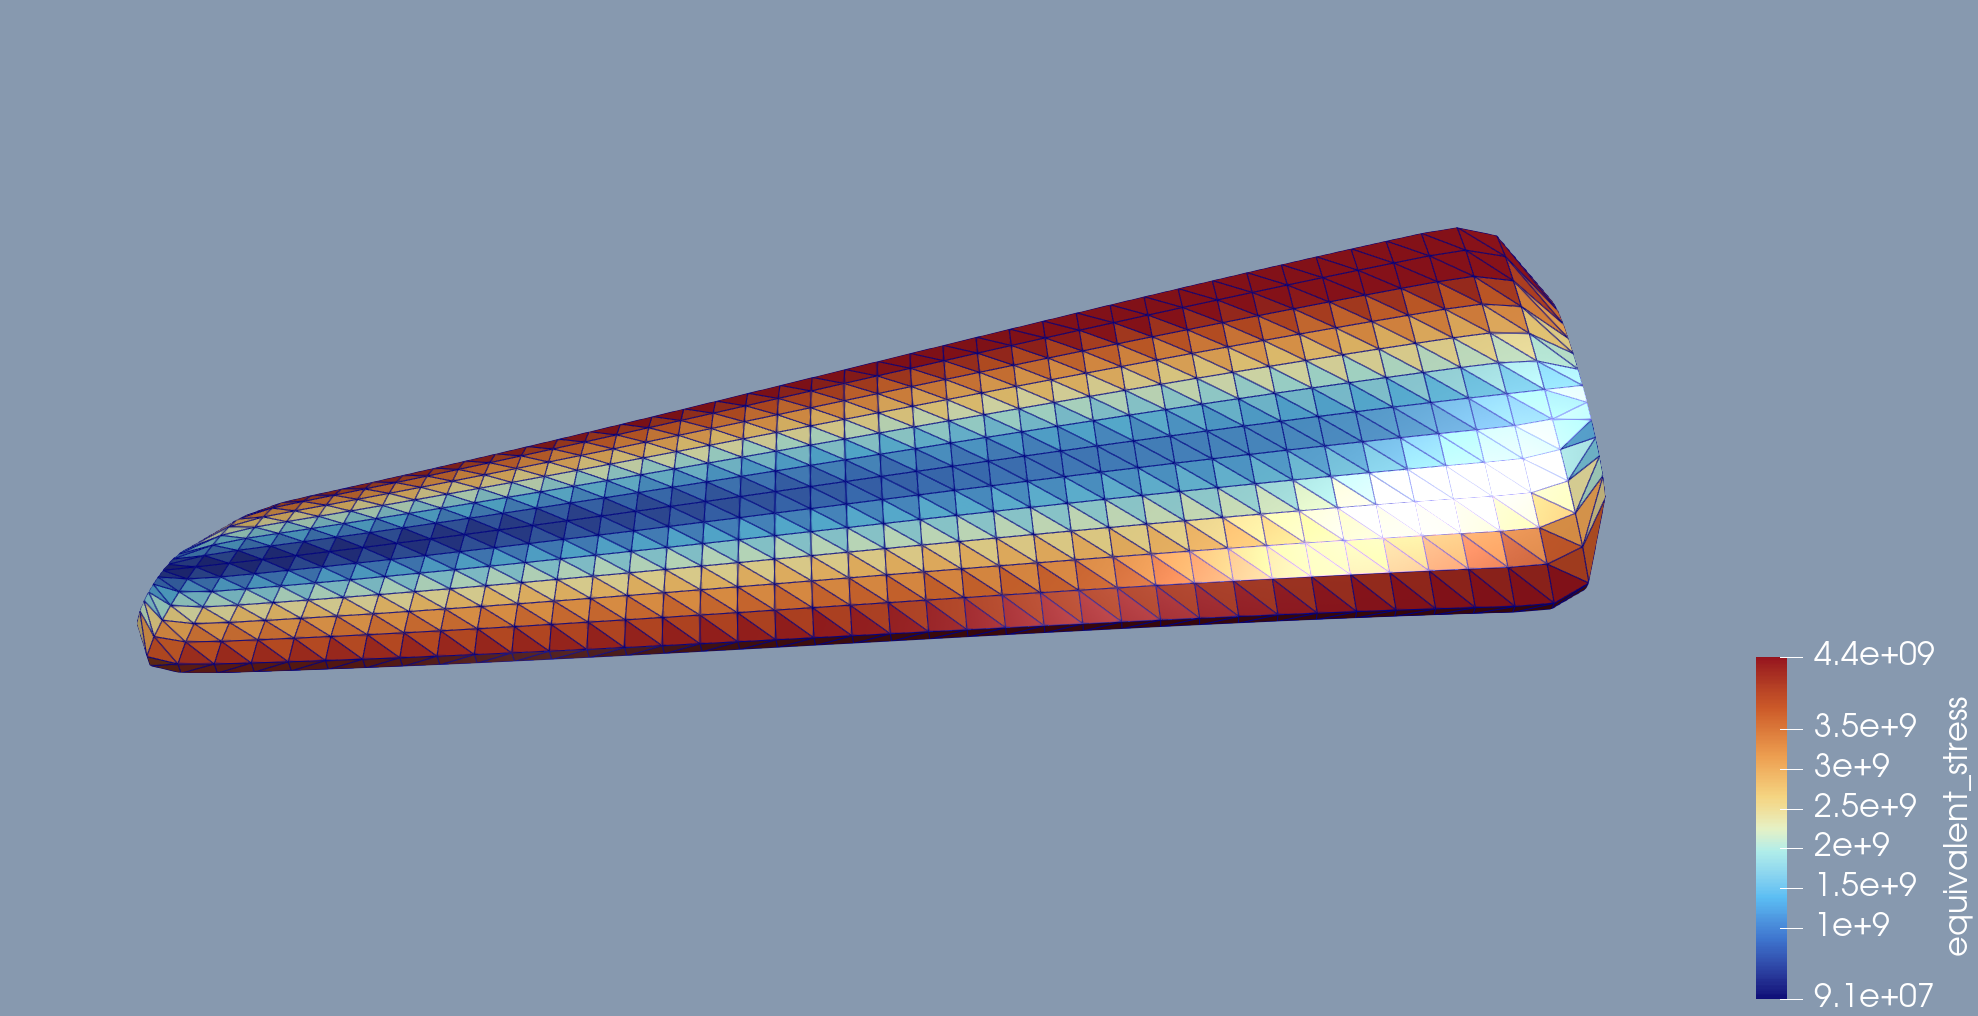
\includegraphics[width=\linewidth]{../images/stress.png}\\[4pt]
        \small Поле $\sigma_{\mathrm{eq}}$ в ParaView
      \end{center}
  \end{columns}
\end{frame}

\begin{frame}{Демонстрация: флаттер в динамике}
  \begin{center}
    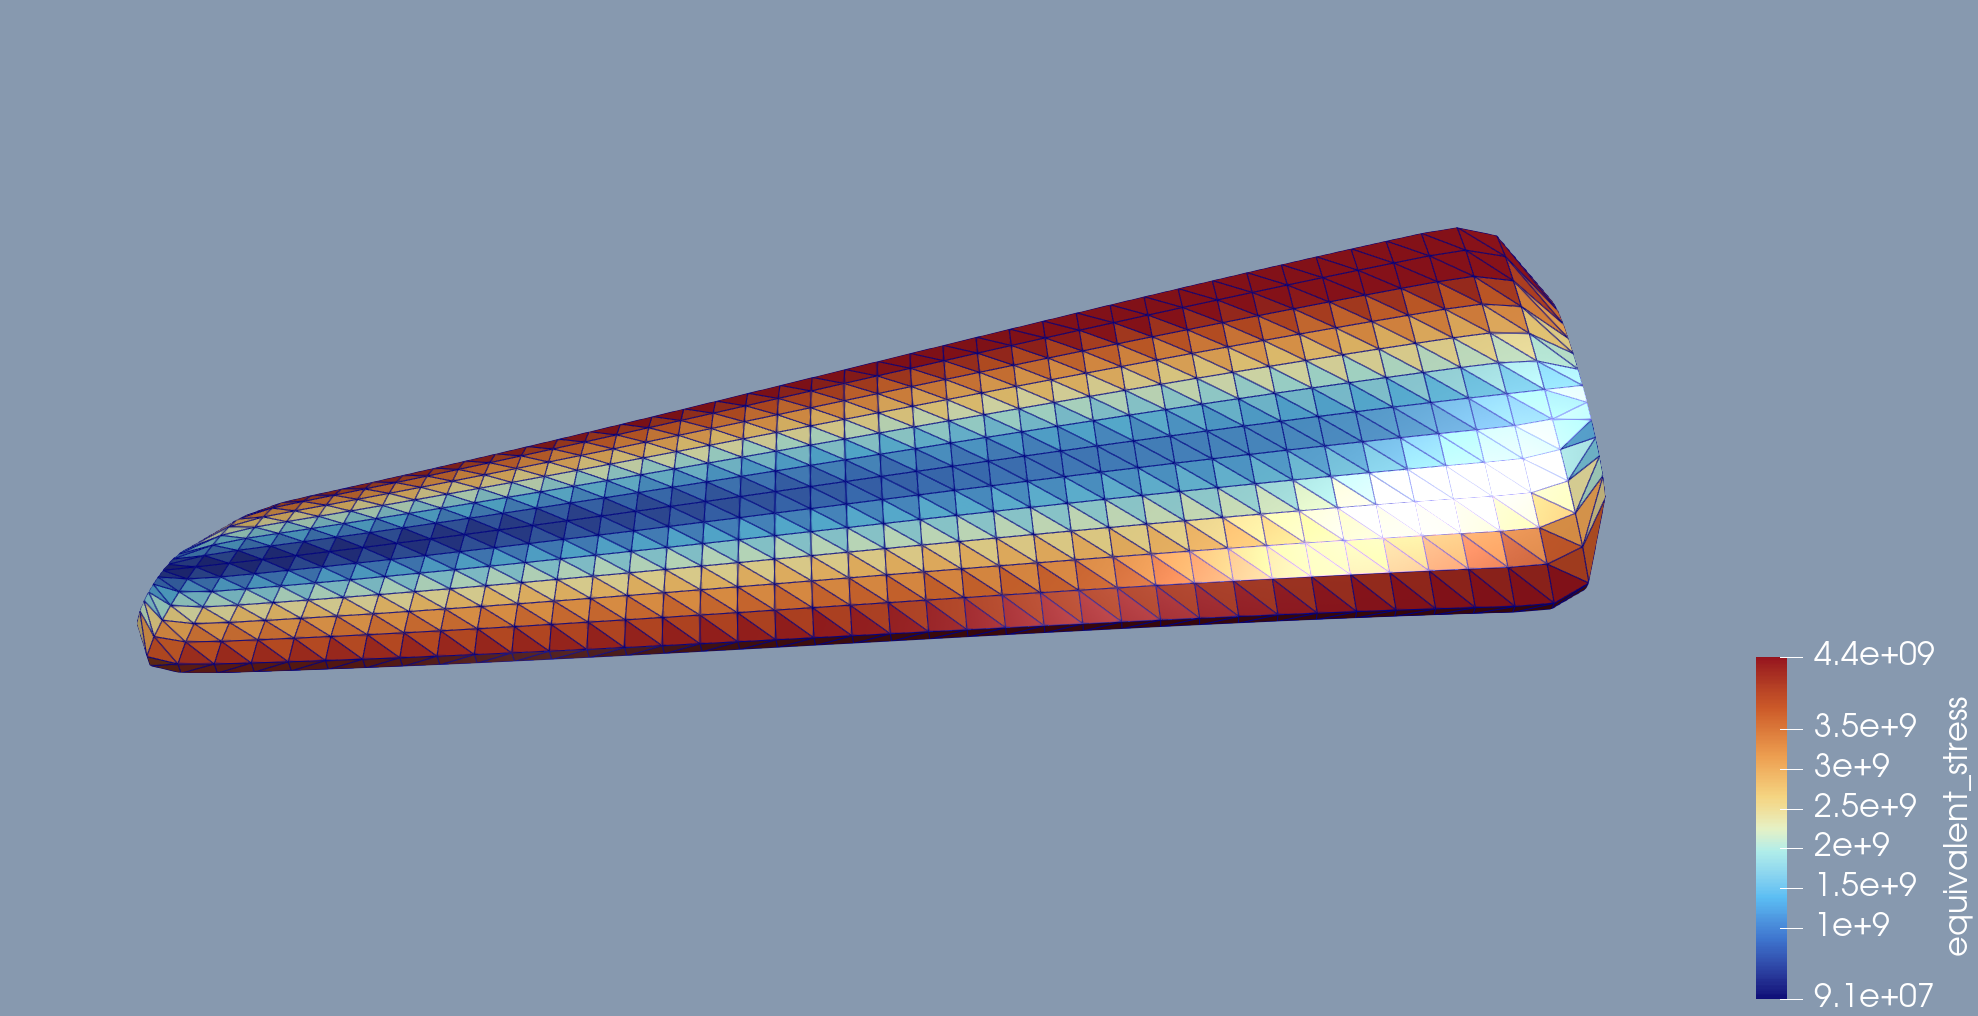
\includegraphics[width=0.72\linewidth]{../images/stress.png}\\[6pt]
    \small Переход от затухающих колебаний к дивергентному флаттеру при $U > U_{\mathrm{crit}}$\\[12pt]
    \href{https://drive.google.com/file/d/1crYL5M6jCOHzeHbBBX5goBmr4ImOLn5Z/view?usp=drive_link}{\beamergotobutton{Анимация}}
  \end{center}
\end{frame}

\begin{frame}{Алгоритм одного временно́го шага}
  \begin{columns}[T]
    \column{0.42\textwidth}
      \begin{block}{Последовательность}
        \begin{enumerate}
          \item Вычислить $\alpha_{\mathrm{eff}}$, $\alpha_{\mathrm{lag}}$
          \item Вычислить $L$ и $M_y$
          \item Интегрировать $\to$ $q_b^{n+1}$, $q_t^{n+1}$
          \item Обновить узлы сетки
          \item Вычислить $\sigma_{\mathrm{eq}}$
          \item Записать VTK-снимок
        \end{enumerate}
      \end{block}

    \column{0.54\textwidth}
      \begin{center}
      \begin{tikzpicture}[
          node distance=0.36cm,
          box/.style={draw=Graphite, fill=GraphiteLight,
                      rounded corners=2pt, font=\scriptsize,
                      text width=4.2cm, align=center, minimum height=0.50cm},
          arr/.style={-{Stealth[length=3.5pt]}, Graphite}
        ]
        \node[box] (a) {Аэродинамические силы};
        \node[box, below=of a] (b) {Изгиб $q_b$};
        \node[box, below=of b] (c) {Кручение $q_t$};
        \node[box, below=of c] (d) {Геометрия (узлы)};
        \node[box, below=of d] (e) {Напряжения $\sigma_{\mathrm{eq}}$};
        \node[box, below=of e] (f) {VTK экспорт};
        \foreach \x/\y in {a/b, b/c, c/d, d/e, e/f}
          \draw[arr] (\x)--(\y);
        \draw[arr, dashed, GraphiteAccent, bend left=65]
          (f.east) to node[right, font=\tiny]{$n{+}1$} (a.east);
      \end{tikzpicture}
      \end{center}
  \end{columns}
\end{frame}

% ══════════════════════════════════════════════════════════════════════════════
\section{Стек, результаты и перспективы}
% ══════════════════════════════════════════════════════════════════════════════

\begin{frame}{Технологический стек и результаты}
  \begin{columns}[T]
    \column{0.48\textwidth}
      \begin{block}{Инструменты}
        \begin{description}
          \item[\textbf{Gmsh}]     тетраэдральная FEM-сетка
          \item[\textbf{C++}]      solver
          \item[\textbf{VTK}]      формат вывода полей
        \end{description}
      \end{block}

      \medskip

      \begin{block}{Достигнуто}
        \begin{itemize}
          \item Изгиб, кручение, напряжения по Мизесу
          \item Все три режима флаттера
          \item Flutter-ready архитектура solver-а
        \end{itemize}
      \end{block}

    \column{0.48\textwidth}
      \begin{block}{Дальнейшее развитие}
        \textit{Аэродинамика:}
        \begin{itemize}
          \item Theodorsen (нестационарная)
          \item Нелинейный $C_L(\alpha)$, срыв потока
        \end{itemize}
        \textit{Конструкция:}
        \begin{itemize}
          \item Геометрическая нелинейность
          \item Критерии разрушения материала
        \end{itemize}
        \textit{Вычисления:}
        \begin{itemize}
          \item Runge-Kutta 4, адаптивный шаг
          \item OpenMP / GPU
        \end{itemize}
      \end{block}
  \end{columns}
\end{frame}

\end{document}
